\newpage
\section{Preliminaries}

Internet technology is the environment in which billions of people and trillions of
devices are interconnected in various ways.
As part of this evolution, Internet becomes the basic carrier
for interconnecting electronic devices – used in industrial
automation, automotive electronics, telecommunications
equipment, building controls, home automation, medical
instrumentation, etc. – mostly in the same way as the Internet came
to the desktops before. More and more devices getting connected to World Wide
Web. Variety of factors have incluenced  this evolutions \cite{4221180}:
\begin{itemize}
\item The availability of affordable, high-performance, low-power
electronic components for the consumer devices. Improved technology can assist
building  advanced functionality into embedded devices and enabling new ways of
coupling between them.
\item Even low cost embedded devices have some wired or wireless interface to local area
networks of the Ethernet type. TCP/IP family protocols are becoming the standard
vehicle for exchanging information between networked devices.
\item The emergence of platform independent data interchange mechanisms based on
Extensible Markup Language (XML) data formatting gives lots of opportunities for developing high-level data interchange and
communication standards at the device level.
\item The paradigm of Web Services  helps to connect various
independent applications using lightweight communications. Clients that are
connected to the service and the service itself may be written using different
programming languages and be executed on different platforms.
\item Presence of Internet allows existing of small embedded controllers and
large production servers in the same network, with a possibility to change
information.
\end{itemize}


The integration of different classes of devices, which employ different
networking technologies, is still an open research area. One of the possible
solutions is the use of SOA software architecture design pattern.



\subsection{Service oriented architecture}
\begin{quote}
Service-oriented computing is a computing paradigm that uses services as basic building blocks for
application development.
\cite {lws_milanovic.pdf}
\end{quote} 

The purpose of \gls{SOA} is to allow easy cooperation of a large number of
computers that are connected over a network.
Every computer can run one or more services, each of them implements one
separate action. This may be a simple business task. Clients can make calls
and receive required data or post some event messages.

Services are self-describing and open components. There is a service interface,
that is based on the exchange of messages and documents using standart formats.
Interface internals ( operating system, hardware platform, programming language)
are hidden from client. Client uses only a service specification scheme, also
called contract. Consumers can get required piece of funcionality by mapping problem
solution steps to a service calls. This scheme provides quick access and easy integration of software components.


Service architecture have been successfully adopted in
business environments. Different information systems, that were created inside
companies for automation of business processes,  are now turned into services
which may easily interact with each other. For example, Estonian goverment uses
services to transmit data between information systems of different departments.
There are also some free services available. Some Internet search companies like
Google, Bing, Yandex provide lots of alternatives how to retrieve data without
using regular browser( search , geolocation and maps,  spell check \gls{API}s )

There are available many techologies which can be used to implement
\gls{SOA}~\cite{wikipedia:SOA}:

\begin{itemize}
  \item Web Services
  \item{SOAP} Simple Object Access Protocol, is a protocol specification for exchanging structured information in the implementation of Web Services in computer networks.
  \item{RPC} Remote procedure call is an inter-process communication that allows
  a computer program to cause a subroutine or procedure to execute in another address space (commonly on another computer on a shared network) without the programmer explicitly coding the details for this remote interaction. 
  \item{REST} Representational state transfer is a style of software architecture for distributed systems such as the World Wide Web. REST has emerged as a predominant web API design model.
  \item{DCOM} Distributed Component Object Model is a proprietary Microsoft technology for communication among software components distributed across networked computers. 
  \item{CORBA}  Common Object Request Broker Architecture enables separate pieces of software written in different
    languages and running on different computers to work with each other like a single application or set of services. Web services
  \item{DDS} Data Distribution Service for Real-Time Systems (DDS) is an Object
  Management Group (OMG) machine-to-machine middleware standard that aims to
  enable scalable, real-time, dependable, high performance and interoperable data exchanges between publishers and subscribers. 
  \item{Java RMI} Java Remote Method Invocation is a Java API that performs the
  object-oriented equivalent of remote procedure calls (RPC), with support for direct transfer of serialized Java objects and distributed garbage collection.
  \item{Jini}  also called Apache River, is a network architecture for the construction of distributed systems in the form of modular co-operating services.
  \item{WCF} The Windows Communication Foundation (or WCF), previously known as
  "Indigo", is a runtime and a set of APIs (application programming interface)
  in the .NET Framework for building connected, service-oriented applications.
  \item{Apache Thrift} is used as a remote procedure call (RPC) framework and
  was developed at Facebook for "scalable cross-language services development".
  \item \ldots
\end{itemize}

This list can be continued. Most of these technologies are inspired by idea

of \gls{RPC}

Web Services are the most popular technology for implementing
service-oriented software nowadays.



 The benefit of SOA is
to allow simultaneous use and easy mutual data exchange between programs of different vendors without additional programming or making changes to the services.

of \gls{RPC}. An \gls{RPC} is initiated by the client, which sends a request
message to a known remote server to execute a specified procedure with specified
parameters. The remote server sends a response to the client, and the application continues its process.

Web Services are the most popular technology for implementing
service-oriented software nowadays. Next section will focus on this framework
and on the main features that any \gls{SOA} implementation should have.
 
\subsection{Web Services architecture}
\subsubsection{Web Services Model}
The Web Services architecture is based on the interactions between three
roles \cite{Kreger2001-WSC}:
service provider, service registry and service requestor. 
This integration has of three operations: publish, find and
bind. The service provider has an implementation of service. Provider defines a
service description and publishes it to a service requestor or service registry.
The service requestor uses a find operation to retrieve the service
description locally or from the service registry and uses the service description to bind with the
service provider and invoke or interact with the Web service implementation.
\autoref{fig:ws_model} illustrates these service roles and their operations.


\begin{center}
 \begin{figure}[H]
	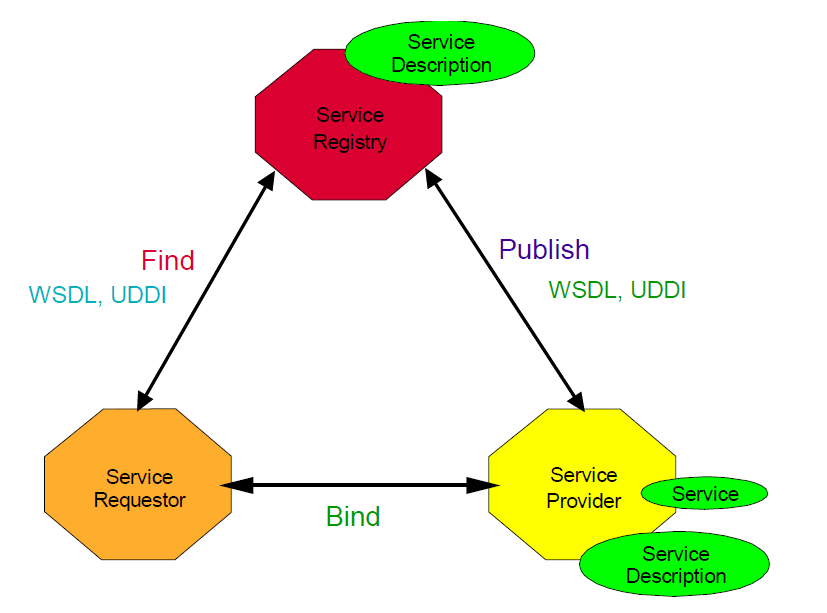
\includegraphics[width=\textwidth]{../images/preliminaries/ws_model.png}
	\caption{Web Services roles, operations and artifacts \cite{Kreger2001-WSC}}
	\label{fig:ws_model}
 \end{figure}
\end{center}

Service registry is a place where service providers can publish
descriptions of their services. Service requestors can find service descriptions
and get binding information from them. Binding can be static and dynamic.
Registry is needed more for dynamic binding where client can get service info at
the runtime, extract necessary functional methods and execute them on the
server. During static binding service description may be directly delivered to
the client at the development phase, for example using usual file, \gls{FTP}
server, Web site, email or any other file transfer protocol.
There are also available special protocols, named Service discovery protocols
(SDP), that allow automatic detection of devices and services on a network. One
of them is the \gls{UDDI} protocol, which is also was mentioned on
\autoref{fig:ws_model}. \gls{UDDI} is shortly described in
\nameref{sec:ws_protocol_stack} section.

\paragraph{\textbf{Artifacts of a Web Service}}
\newline
Web service consists of two parts~\cite{Kreger2001-WSC}:
\begin{itemize} 
\item \label{itm:service_description_artifact} 
\textbf{Service Description}~~~The
service description contains the details of the interface and implementation of the service. This includes its data types, operations, binding
information and network location. There could also be a categorization and
other metadata about service discovery and utilization. It may contain some
Quality of service (QoS) requirements. 

 \item \textbf{Service}
 ~~~This is the implementation of a service - a software module deployed on network accessible platforms provided by the service provider.
 Service may also be a client of other services. Implementation details
 are encapsulated inside a service, and client does not know the details how
 server processes his request.
\end{itemize}



\subsubsection{Web Services Protocol Stack}
\label{sec:ws_protocol_stack}

WS architecture uses many layered and interrelated technologies.
\autoref{fig:ws_protocol_stack} provides one illustration of some of these technology families.

\begin{center}
 \begin{figure}[h]
	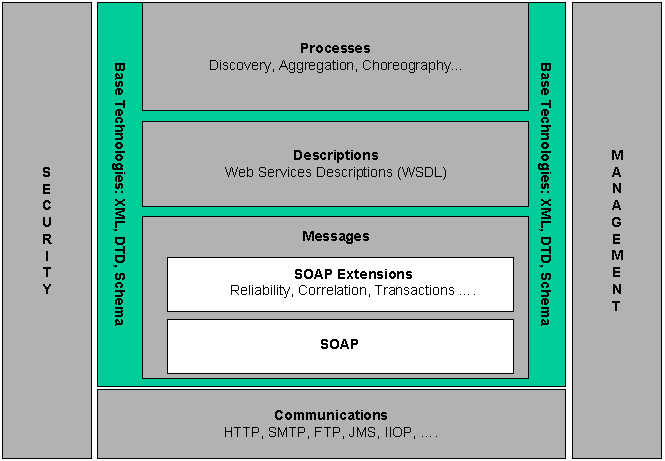
\includegraphics[width=\textwidth]{../images/preliminaries/ws_protocol_stack.png}
	\caption{Web Services Architecture Stack \cite{ws_arch} }
	\label{fig:ws_protocol_stack}
 \end{figure}
\end{center}

We can describe these different layers as follows:
\begin{itemize}
  \item \textbf{Communications} - This layer represents a transport between
  communication parties( service provider, client, service registry). This layer
  can be any network protocol like: \gls{HTTP}, \gls{FTP}, \gls{SMTP} or any
  other suitable transport protocol. If Web service is used in the Internet, the
  transport protocol in most cases will be \gls{HTTP}. In internal networks there is the opportunity to agree upon the use of alternative
network technologies.

\item \textbf{Messages} - In order to communicate with a service, client should
send a message. Messages are \gls{XML} documents with different structure.
\gls{SOAP} protocol defines how these messages should be structured.
\gls{SOAP} is implementation independent and may be composed using any
programming language. Protocol specification and message descriptions can be
found in document SOAP Version 1.2 Part 1: Messaging Framework (Second
Edition)\cite{soap_protocol_spec}.

\item \textbf{Descriptions} - This layer contains the definition of service
interface (see also \autoref{itm:service_description_artifact}). Web Services
use \gls{WSDL} language for describing the functionality offered by a service.
\gls{WSDL} file is the contract of service, which contains information about how
the service can be called, what parameters it expects, and what data structures it returns.
It is similar to method signatures in different programming languages.

\item \textbf{Processes} - This part contains specifications and protocols
about how service could be published and discovered. Web services are meaningful
only if potential users may find information sufficient to permit their execution.
Service as a software module has its own lifecycle, it needs to be deployed and deleted somehow.
Traditional Web Services use \gls{UDDI}  mechanism to register and locate web
service applications. \gls{UDDI} was originally proposed as a core Web service
standard.
<<<<<<< HEAD
 
=======

\item \textbf{Security} -

\item \textbf{Management} -
>>>>>>> 598d0d163e44a3ede03fc09c18b9a7f519a19979
\end{itemize}

\subsubsection{Basic Service Description and Service Contract}
\label{sec:ws_service_contract}
\gls{WSDL} file is an \gls{XML} document which has specification of  service contract.
As it was mentioned earlier(\autoref{itm:service_description_artifact}) contract should be shipped with a component and should  tell the
client what input does service expect, and what output it will produce if specified input conditions are met. 
Contract may be a primary specification and it should be enough for a client to start using a service.
This is similar to library header file in C language. 
You have a ready and compiled library shipped with a header file, where are all method declarations and definitions of data strutures. 
If header file is verbose enough, there is no need to use the documentation. You can place this component into your system very easily.



Regular \gls{WDSL} document contains some necessary elements ~\cite{wsdl_language_spec, wikipedia:WSDL}:


\begin{table}[h]
	\centering	
	\begin{tabular}[h]{|l|l|}
		\hline
		\textbf{WSDL 2.0 Term} & 
		\textbf{Description} 	
	    	\tabularnewline
		\hline
			Service &
			The service element describes \textit{where} to access the service. 
			A WSDL 2.0 service specifies a single interface that the service will support,
			and a list of endpoint locations where that service can be accessed.
			
			
	    	\tabularnewline	    	
	    	\hline
			Endpoint & 
			Defines the address or connection point to a Web service. 
			It is typically represented by a simple HTTP URL string.
			Each endpoint must also reference a previously defined binding to indicate 
			what protocols and transmission formats are to be used at that endpoint.
				
	    	\tabularnewline

	    	\hline
			Binding &		
			Specifies concrete message format and transmission protocol details for an interface, and must supply such details for every operation and fault in the interface.
	    	\tabularnewline

	    	\hline
			Interface &
			Defines a Web service, the operations that can be performed, and the messages that are used to perform the operation.
			Defines the abstract interface of a Web service as a set of abstract \textit{operations},
			each operation representing a simple interaction between the client and the service. 
			Each operation specifies the types of messages that the service can send or receive as part of that operation.
			Each operation also specifies a message exchange \textit{pattern} that indicates the sequence in which the associated messages are to be transmitted between the parties. 
	    	\tabularnewline

		\hline
			Message Types &
			The types element describes the kinds of messages that the service will send and receive.
			The XML Schema\footnote{XML schema is the XML document, that specifies structure of other XML document and describes data types and constraints,
			that other document might have. 
			You can create a schema for necessary XML data structure and verify if processed message corresponds to schema you have already defined}
			language (also known as XSD) is used (inline or referenced) for this purpose.
	    	\tabularnewline


		\hline
	  
	\end{tabular} 
	\caption{Objects in WSDL 2.0~\cite{wsdl_language_spec, wikipedia:WSDL} }
	\label{tbl:wdsl_members}
\end{table} 


Document may also contain optional element named \textit{documentation}.
There may be human readable service documentation, with   purpose and use of the service, the meanings of all messages, constraints their use, and the sequence in which operations should be invoked.
To be documentation more complete, you may specify an external link to any additional documentation.

SOMETHING ELSE ABOUT CONTRACTS

\subsection{SOA and Embedded Systems}


\subsubsection{Authentication and Authorization in embedded systems}
\paragraph{Need of security}
Authorization is the process of granting or denying access to a network resource.
Most computer security systems are based on a two-step process.
The first stage is authentication, which ensures that a user is who he or she claims to be.
The second stage is authorization, which allows the user access to various resources based on the user's identity. 

Users are essential part of every system. System should be designed with
a requirement, that there will be at least one user. System without any purpose
does not make sense. Usually information systems have lots of users with
different roles. There should be an system administrator - the most authorized individual
in the system, managers and normal users. System should distinct them all
somehow. 

Another requirement is system and information security. System may contain
sensitive data, that should not be available to general users. In case of remote
services there are some services that are not open. These services or some
of their parts are require some identity to pass through. 

Let's take a usual website as example. Common website has at least three
different user roles:
user or guest, content publisher and system administrator. Last two roles may be
joined together, but in general content publishers do not do system maintenance, they
just work with content of webpages. There may be more different roles, but these
are the main ones. Imagine you open a web page and you see the content. You
follow the links and surf the web site. If you want to change something, for
example you do not like the design or some words on web page were misspelled,
you need to find special place where you can input your \textbf{credentials} and
get into the system. This will happen only if you have proper
\textbf{permission} to do that. When you get inside you are still not able to do
anything due to lack of privileges. For example you cannot turn of the
webserver or disable the your website. There may be lots of different roles and
responsibilities in the system and each role has limited access to system
resources.

Embedded device as a service may be similar to system example above. Device may
have some limited use cases, that are not available to not authorized service
clients. This may be internal information retrieving, some  device
manipulation functions (turn on/off something, delete/remove something from the
system, change of system preferences). Some device functionality may be
available only for limited people, for example system owner. The real life example of such system is the wireless
router. Router clients are other computers, they can send and receive network
packets. Router uses wireless security protocols, which permit unauthorized
access. Even if you are connected to a secure access point, you are not able to
change system settings. You should have admin permission (password) to manage
the system. This kind of system, like many embedded systems, is made for one
purpose. Router purpose is to provide access for the network. You also can
remember lots of similar systems, that use authorized access. Nowadays it is not new to get
remotely into some device and to change internals, but embedded system
integrations are still not so common. Imagine near future, you are sitting at
work and thinking to go home. After a long day you became really hungry. You
take your smartphone and connect to your remote wireless fridge service at home. You type
your password and get list of all food in your fridge. Now you know what you
need to buy and the real candidates to be throwed to the rubbish bin. You adjust
power in some fridge area and your beer will be very cold when you get home. Is
it just a dream? Is it really hard to realize using present time technologies?


The main problem here is the security. Wired embedded network protocols are
mostly not designed with security in mind. These networks were isolated from the
Internet in the past. They could only be attacked using direct physical access
to the network. Nowadays Internet and wireless networks are popular. Lots of
communication between different systems goes through the wireless channel. Radio link is also available to your neighbour behind the wall. Generally, you do not want to broadcast what is in your fridge or to give ability to connect to your air conditioning service. Therefore you need to use some authentication scheme for
your service.

\paragraph{Authentication protocols}

Authentication is any process by which you verify that someone is who they claim
they are. (https://httpd.apache.org/docs/2.2/howto/auth.html)

Humanity has already invented a lot of different authentication techniques. 

The ways in which someone may be authenticated fall into three
categories: (http://en.wikipedia.org/wiki/Authentication)
\begin{itemize}
  \item the ownership factors: Something the user has (e.g., wrist band, ID
  card, security token, software token, phone, or cell phone)
  \item the knowledge factors: Something the user knows (e.g., a password, pass
  phrase, or personal identification number (PIN), challenge response (the user must answer a question), pattern)
  \item the inherence factors: Something the user is or does (e.g., fingerprint,
  retinal pattern, DNA sequence (there are assorted definitions of what is sufficient), signature, face, voice, unique bio-electric signals, or other biometric identifier).
\end{itemize}

Authentication may be one way (only client is checked for validity) and two way
( both client and server check each other). Some systems  may requre to use
different security factors together: you say password, provide ID card and show
you fingerprint There are also available many standard authentication protocols.
If you start searching you will probably find similar list:
\begin{itemize}
  \item Transport Layer Security (TLS)
  \item Extensible Authentication Protocol (EAP)
  \item Password authentication protocol (PAP)
  \item Challenge-Handshake Authentication Protocol (CHAP)
  \item Password-authenticated key agreement
  \item Remote Authentication Dial In User Service (RADIUS)
  \item Kerberos
  \item Lightweight Extensible Authentication Protocol (LEAP)  
\end{itemize}

Choosing suitable protocol is not trivial problem. There is no any case general
protocol.  Most of them are designed to interconnect big computers inside a
network. Mostly they operate on transport and application level and use TCP/IP
protocol stack.

All these protocols could be devided into these groups:
\begin{itemize}
  \item Protocols that transmit the secret over the network. (For example
  Password authentication protocol). These protocols are not secure.
  \item Protocols that not send secrets and provide authentification through
  sending messages. (CHAP and Password-authenticated key agreement).
  \item Protocols that require a trusted third party.  
\end{itemize}

Protocols of first type have been deprecated because of security reasons. They
send sensitive data over the network and everyone else between two nodes can
catch this data.

Second group of protocols was invented because the first group was unable to
provide proper level of security. Link between client and server (two parties)
does not contain pure information about the secret. Parties use cryptography and
send encrypted messages to each other. Finally they authenticate each other when there is enough information gathered to validate the authority.

Last group uses trusted third party authority to check each other. There is
assumption that all three parties should have connection between each other. Embedded device during
client authentification needs to connect some server and ask for a secret. Third
party should always have a high authority, two other parties should trust him.
This scheme should be used in case of high security requirements.



Choosing of right authentication protocol in general should depend on application.
Sometimes, there will be enough just to send plain text passwords over the
network.
Engineer should analyze all hazards during system design process.

Lifecycle of an embedded system is more longer than livecycle of average personal computer. Application specific controller  may run for decades and it will be still functional.
Choosed security algorithm may be not secure enough after some years. Some vulnerabilities can be discovered during that period. 
Computational power of modern processors raises every year and  secure encryption may be cracked during some seconds in the future.
There is no 100\% secure system, everything can be breaked. 

Your system security should have such encryption, that provides proper security
level to your application data and can not be cracked quickly.
How quick it is depends on your data and security requirements of your data.

Another aspect is the complexity of cryptography algorithms. Embedded devices
are usually small low power devices with limited computation abilities. Not
every algorithm suits well. It should be quick and resource friendly , and in
same time it should be secure.

Nowadays, the last versions of the Wifi and Wimax standards include the use of
Extensible Authentication Protocol (EAP) declined in different versions
(LEAP - EAP using a Radius Server -, EAP-TTLS, etc...). In practice, EAP is interesting for workstations or desktop computers but does not fit the needed security of particular systems such as handheld devices, short-range communication sys- tems or even domestic Wireless LAN devices. The reason being that many versions of EAP use certificates,
public key encryption or exhaustive exchanges of information, that are not viable for lightweight wireless
devices.[A new generic 3-step protocol for authentication and key
agreement in embedded systems]

Protocol should small in code size. You should not to place a
separate controller, which deals with communication,  into your system.
Everything is needed to be inside one small and cheap device. Business requires
as low price as possible, because only that it could give you any money.


Embedded networking has constraints that developer should keep in mind
while developing a system.

% There are already available small realizations of TCP/IP stack that could be run
% [ssylka na doktorskuju Programming
% Memory-Constrained
% Networked Embedded Systems] on small 8-bit microcontrollers, but they have only
% limited protocol stack and security protocols need to be provided separately.
% 
% There are  

\paragraph{Embedded Network Constraints} [A Flexible Approach to Embedded Network
Multicast Authentication]
Embedded networks usually consist of a number of Electronic Control
Units (ECUs). Each ECU performs a set of functions in the system. These ECUs are
connnected to a network, and communicate using a protocol such as CAN,
FlexRay, or Time-Triggered Protocol (TTP). These protocols are among the most
capable of those currently in use in wired embedded system networks. Many other protocols are even
less capable, but have generally similar requirements and constraints:

\begin{itemize}
  \item{Multicast Communications} - All messages sent on a
distributed embedded network are inherently multicast,
because all nodes within the embedded system need to
coordinate their actions. Once a sender has transmitted a
packet, all other nodes connected to the network receive the
message. (In CAN, hardware performs message filtering at the
receiver based on content.) Each packet includes the sender's
identity, but does not include explicit destination information. The configuration of the network is
usually fixed at design time, and changes a littel or  does not change at all.
\item{Resource Limited Nodes} - 
Processing and storage capabilities
of nodes are often limited due to cost considerations at design
time. Controllers, that are used usually have no more than 32 kilobytes of RAM
and 512 kilobytes of Flash memory. Their operating frequency is no more than 100
MHz. Authentication mechanisms which require large amounts of
processing power or storage in RAM may not be feasible.
\item{Small Packet Sizes} - Packet sizes are very small in embedded
network protocols when compared to those in enterprise
networks. The bandwidth is very limited. Network synchronization and packet
integrity checks should be added to this. For example data rates are limited to
1 Mbit/sec for CAN and 10 Mbit/sec for TTP and FlexRay. Devices cannot store
large packets in memory during processing, as it was mentioned in previous
requirement. Authentication should have minimal bandwidth overhead.
\item{Tolerance to Packet Loss} - Embedded systems often work in a
very noisy environment. Data may corrupt during transmission. Authentication
schemes must be tolerant to packet loss.
\item{Real-Time Deadlines} - In real-time safety-critical systems, delays are
not tolerated. Processes should be completed within specified deadlines.
Authentication of nodes must occur within a known period of time. There should
not be unspecified delays.
\end{itemize}


\paragraph{Challenge-Handshake Authentication}

In this work i decided to use Challenge-Handshake Authentication Protocol
[http://tools.ietf.org/html/rfc1994].

CHAP is an authentication scheme used by Point to Point Protocol (PPP) servers to validate the identity of remote clients. 
CHAP periodically verifies the identity of the client by using a three-way handshake. 
This happens at the time of establishing the initial link (Link control protocol), and may happen again at any time afterwards.
The verification is based on a shared secret (such as the client user's
password).
\begin{enumerate}
  \item After the completion of the link establishment phase, the authenticator
  sends a "challenge" message to the peer.
  \item The peer responds with a value calculated using a one-way hash function
  on the challenge and the secret combined.
  \item The authenticator checks the response against its own calculation of the
  expected hash value. If the values match, the authenticator acknowledges the authentication; otherwise it should terminate the connection.
  \item At random intervals the authenticator sends a new challenge to the peer
  and repeats steps 1 through 3.
\end{enumerate}

The secret is not sent over the link.
Although the authentication is only one-way, you can negotiate CHAP in both directions, 
with the help of the same secret set for mutual authentication.

This protocol is described in the document [http://tools.ietf.org/html/rfc1994].
Document specifies main protocol consepts and packet formats.

There are some procol extensions like MS-CHAP and CHAP is used
as a part of other protocols like EAP(EAP MD5-Challenge) and RADIUS (uses CHAP
packets). They all use CHAP concepts somehow. 

One of the main puproses of this work is to develop a prototype of an embedded
service. This system uses JSON [SEEE JSON SECTION] object format to encapsulate
pieces of information. I will port CHAP packet format to JSON object. It need to
be the same CHAP protocol but it should be placed into JSON. See
[CHAP IMPLEMENTATION SECTION] for more details.



\paragraph{Conclusion}

Information security is continuing process. There are lots of scientist all
over the world, that are trying to invent new approaches how to protect data.

In the Internet-connected future, designers will have to port existing
security approaches to embedded control systems. This requires the use of 
lightweight security protocols.

Embedded control and acquisition devices may be integrated to the main
infrastructure of the several sorganisation. These connections need to be secure
enough.
Resent decades ago Internet was also a research project, and top computers were
like nowadays microcontrollers are. But now it is used in whole world as one of
the main communication methods. Even banks are using it for transactions. There are
lots of security schemes with different level of protection. I believe that
even small 8-bit microcontroller can be securely connected to World Wide Web it
the near future.



\subsection{Data serialization}
\subsubsection{JSON}
\subsubsection{XML}
\subsubsection{Others}